%% LyX 2.0.6 created this file.  For more info, see http://www.lyx.org/.
%% Do not edit unless you really know what you are doing.
\documentclass[12pt,english]{paper}
\usepackage{lmodern}
\renewcommand{\sfdefault}{lmss}
\renewcommand{\ttdefault}{lmtt}
\usepackage[T1]{fontenc}
\usepackage[latin9]{inputenc}
\usepackage{geometry}
\geometry{verbose,tmargin=2.8cm,bmargin=2.8cm,lmargin=2.8cm,rmargin=2.8cm}
\usepackage{babel}
\usepackage{calc}
\usepackage{url}
\usepackage{amsthm}
\usepackage{amsmath}
\usepackage{amssymb}
\usepackage{graphicx}
\usepackage{esint}
\usepackage[unicode=true,pdfusetitle,
 bookmarks=true,bookmarksnumbered=false,bookmarksopen=false,
 breaklinks=false,pdfborder={0 0 1},backref=false,colorlinks=false]
 {hyperref}

\makeatletter

%%%%%%%%%%%%%%%%%%%%%%%%%%%%%% LyX specific LaTeX commands.
%% A simple dot to overcome graphicx limitations
\newcommand{\lyxdot}{.}


%%%%%%%%%%%%%%%%%%%%%%%%%%%%%% Textclass specific LaTeX commands.
\newcommand{\lyxaddress}[1]{
\par {\raggedright #1
\vspace{1.4em}
\noindent\par}
}
\theoremstyle{plain}
\newtheorem{thm}{\protect\theoremname}[section]

\@ifundefined{showcaptionsetup}{}{%
 \PassOptionsToPackage{caption=false}{subfig}}
\usepackage{subfig}
\makeatother

\providecommand{\theoremname}{Theorem}

\begin{document}

\title{The Normal Distribution from Gauss to Kalman}


\author{Divakar Viswanath}

\maketitle

\lyxaddress{Department of Mathematics, University of Michigan}


\date{November 2014}

\tableofcontents{}


\section{Introduction: random variables, expectation/mean, and variance}

In this lecture, we will introduce the normal distribution, which
is one of the great ideas in mathematics. Its applicability is very
wide, touching every area of the sciences. In addition, there are
mathematical questions related to it that are still a subject of active
research.

To gain an understanding of the normal distribution, we will begin
with a simple example and rigorously deduce the central limit theorem
for that example. The central limit theorem gives a partial explanation
of why the normal distribution occurs in so many situations. 

Our next step is to deduce a very special case of the Kalman filter.
The Kalman filter is one of the most consequential ideas in applied
mathematics. Its applications are profound. The cell phone in your
pocket may have a Kalman filter. Although I have no direct knowledge,
I am certain that India's Mars mission Mangalyaan makes extensive
use of Kalman filters. 

The Kalman filter is a method for the systematic calculation of means
and variances. So we will begin by understanding random variables,
means or expectations, and variances.

\begin{figure}
\begin{centering}
\includegraphics[scale=0.5]{\lyxdot \lyxdot /figs/heights}
\par\end{centering}

\caption{Normal law fit to the height distribution of 1078 subjects (fathers)
in Pearson's data set.\label{fig:intro-heights-normal-law}}


\end{figure}


Figure \ref{fig:intro-heights-normal-law} provides motivation for
our study of the normal law. The figure has two items in it. The first
item is a histogram. The heights of 1078 fathers (as well as their
sons, but we ignore the sons) were recorded by the eminent statistician
Karl Pearson. The minimum recorded height was $59$ inches (which
is an inch short of $5$ feet) and the maximum was $75.4$ inches
(which is $3.4$ inches above $6$ feet). To obtain this histogram,
this range of heights is divided into $15$ bins so that every bin
is approximately an inch. The vertical axis of the figure shows the
number of persons in each bin.

The second item in Figure \ref{fig:intro-heights-normal-law} is the
normal fit to the heights data. As you can see the fit is good but
not very accurate. The convergence to the normal law is quite slow,
typically at the rate $n^{-1/2}$ if the number of data points is
$n$. We will understand Figure \ref{fig:intro-heights-normal-law}
better as we progress in this lecture, but as far as I am aware there
are still many things in it that are yet not understood.
\begin{description}
\item [{Note:}] The source for this document as well as the python programs
used to produce the figures are posted at \url{https://github.com/divakarvi/14-kvpy}
\end{description}

\subsection{Random variables}

The random variable is a mathematical abstraction of phenomena that
we cannot calculate perfectly. The complete definition of a random
variable is a little complicated. The difficulties in defining a random
variable are related to the difficulties in defining a set axiomatically.
We will not go into those difficulties. Instead, we assume that the
notion of a random variable $X$ is a given. That means that for any
set $A$, we know the probability 
\[
\mathbb{P}\left(X\in A\right).
\]


Certain random variables are discrete. That means they take values
in a finite set $\left\{ a_{1},\ldots,a_{M}\right\} $ or a countable
set. For example, $X$ may take only the two values $\pm1$. In that
case if we give the probabilities $\mathbb{P}(1)$ and $\mathbb{P}(-1)$
then we have specified the random variable completely. The probabilities
must of course sum to $1$. 

Certain other random variables may be specified in terms of a continuous
probability density function $p(x)$, where $x\in\mathbb{R}$. In
this case,\texttt{
\[
\mathbb{P}\left(a\leq X\leq b\right)=\int_{a}^{b}p(x)\, dx.
\]
}We require the normalization condition $\int_{-\infty}^{\infty}p(x)\, dx=1$. 

Notice that discrete random variables cannot be represented using
densities. That problem can be dealt with fairly easily by passing
to the Stieltjes integral, which is the next step from the Riemann
integral. One can make up examples of random variables that cannot
be represented using the Stieltjes integral. Modern definitions of
random variables rely upon the Lebesgue theory and its extensions.

The probability density function $p(x,y)$ represents two random variables
$X,Y$ simultaneously. It is assumed to be continuous. We have 
\begin{eqnarray*}
\mathbb{P}\left(a\leq X\leq b,\, c\leq Y\leq d\right) & = & \int_{c}^{d}\int_{a}^{b}p(x,y)\, dx\, dy\\
\mathbb{P}\left(a\leq X\leq b\right) & = & \int_{-\infty}^{\infty}\int_{a}^{b}p(x,y)\, dx\, dy\\
\mathbb{P}\left(c\leq Y\leq c\right) & = & \int_{c}^{d}\int_{-\infty}^{\infty}p(x,y)\, dx\, dy.
\end{eqnarray*}
The normalization condition here is that $\int_{-\infty}^{\infty}\int_{-\infty}^{\infty}p(x,y)\, dx\, dy=1$.
We can obtain the density functions of $X$ and $Y$ as
\begin{eqnarray*}
p_{X}(x) & = & \int_{-\infty}^{\infty}p(x,y)\, dy\\
p_{Y}(y) & = & \int_{-\infty}^{\infty}p(x,y)\, dx.
\end{eqnarray*}
In the same manner, we can consider joint density functions for any
finite number of random variables. 

The joint density function holds information about how the random
variables are related to each other. If much of the mass of the density
function $p(x,y)$ is concentrated near the diagonal $x=y$, then
the random variables $X$ and $Y$ are highly correlated and take
nearly the same value much of the time.

\emph{Independence }is one of the key concepts. The random variables
$X$ and $Y$ are independent if 
\[
\mathbb{P}\left(X\in A\:\text{and}\: Y\in B\right)=\mathbb{P}\left(x\in A\right)\mathbb{P}\left(y\in B\right),
\]
where $A$ and $B$ are any two sets. Similarly, $X_{1},\ldots,X_{n}$
are an independent sequence of random variables if 
\[
\mathbb{P}\left(X_{1}\in A_{1},\ldots,X_{n}\in A_{n}\right)=\prod_{i=1}^{n}\mathbb{P}\left(X_{i}\in A_{i}\right).
\]
The random variables represented by the density function $p\left(x_{1},\ldots,x_{n}\right)$
are independent if $p\left(x_{1},\ldots,x_{n}\right)=p_{1}\left(x_{1}\right)p_{2}\left(x_{2}\right)\ldots p_{n}\left(x_{n}\right)$.
They are independent and identically distributed if 
\[
p\left(x_{1},\ldots,x_{n}\right)=p(x_{1})p(x_{2})\ldots p(x_{n}).
\]
The definition of independence extends to discrete random variables
as well.


\subsection{Mean or expectation}

If $X$ is a discrete random variable that takes the values $a_{1},\ldots,a_{M}$
with probabilities $p_{1},\ldots,p_{M}$, respectively, then its mean
is given by 
\[
\frac{p_{1}a_{1}+\cdots+p_{M}a_{M}}{M}.
\]
In the mathematical literature, the mean is called expectation or
expected value and denoted $\mathbb{E}X$. If the random variable
is represented using the density function $p(x)$, then we have 
\[
\mathbb{E}X=\int_{-\infty}^{\infty}xp(x)\, dx.
\]
If $f(\cdot)$ is a suitable function, then we have $\mathbb{E}f(X)=\int_{-\infty}^{\infty}f(x)\, p(x)\, dx.$

If $X_{1},\ldots,X_{n}$ are a sequence of random variables then we
may prove that 
\[
\mathbb{E}\left(X_{1}+\cdots+X_{n}\right)=\mathbb{E}X_{1}+\cdots+\mathbb{E}X_{n}.
\]
The proof does not assume that the $X_{i}$ are independent.
\begin{description}
\item [{Exercise:}] Prove the above identity assuming the random variables
$X_{1},\ldots,X_{n}$ to be represented by the density function $p\left(x_{1},\ldots,x_{n}\right)$.
You may assume the existence of all integrals that arise.
\item [{Exercise:}] Let $\pi_{1},\ldots,\pi_{n}$ be a random permutation
of the numbers $1,\ldots,n$ which is equally likely to be any one
of the $n!$ possible permutations. We say that the permutation has
a descent at the position $i$ if and only if $\pi_{i}>\pi_{i+1}$.
A permutation may have $d$ descents with $0\leq d\leq n-1.$

\begin{itemize}
\item Find the permutation with $0$ descents. 
\item Find the permutation with $n-1$ descents.
\item Prove that the expected number of descents is $(n-1)/2$.
\end{itemize}



\item [{Exercise:}] Give an example of a random variable whose expectation
is $\infty$. Give an example of a random variable whose expectation
does not exist.
\item [{Exercise:}] If $X$ and $Y$ are independent random variables and
may be represented using a density function, prove that $\mathbb{E}XY=\mathbb{E}X\:\mathbb{E}Y$,
assuming all integrals that arise to exist.
\item [{Exercise:}] If $X$ and $Y$ are independent random variables and
may be represented using a density function, as above, and $f$ and
$g$ are any continuous functions prove that 
\[
\mathbb{E}f(X)g(Y)=\mathbb{E}f(x)\:\mathbb{E}g(Y).
\]
You may assume that all functions that arise in the calculation are
integrable.
\end{description}

\subsection{Variance and standard deviation}

If we know only the mean of a random variable, we know practically
nothing about it. If we know its mean and its standard deviation,
we have a great deal of information, as we will soon understand. What
then is standard deviation?

The standard deviation, or the variance which is the square of the
standard deviation, quantifies the typical size of fluctuations. If
$\mathbb{E}X=\mu$, then the variance $\sigma^{2}$ of $X$ is defined
as 
\[
\sigma^{2}=\mathbb{E}\left(X-\mu\right)^{2}.
\]
The standard deviation is $\sigma$. It is often called the root-mean-square
value since it is given by $\sqrt{\mathbb{E}\left(X-\mu\right)^{2}}$. 
\begin{description}
\item [{Exercise:}] Prove that $\sigma^{2}=\mathbb{E}X^{2}-\left(\mathbb{E}X\right)^{2}$. 
\item [{Exercise:}] Give an example of a variable whose mean is finite
and standard deviation infinite.
\end{description}

\subsection{The normal distribution}

The density function of the standard normal distribution is given
by 
\begin{equation}
\frac{1}{\sqrt{2\pi}}\exp\left(-x^{2}/2\right).\label{eq:intro-std-normal}
\end{equation}
It is properly normalized because 
\[
\frac{1}{\sqrt{2\pi}}\int_{-\infty}^{\infty}\exp(-x^{2}/2)\, dx=\frac{1}{\sqrt{\pi}}\int_{-\infty}^{\infty}\exp(-x^{2})\, dx=1.
\]
This latter integral (called Gaussian integral) was first evaluated
by Laplace. The popular method for evaluating it using double integrals
and polar coordinates (see the wikipedia article \url{http://en.wikipedia.org/wiki/Gaussian_integral})
is due to Poisson and based on an earlier method of Laplace. 

Given the Gaussian integral, it follows that 
\begin{equation}
\frac{1}{\sqrt{2\pi}}\int_{-\infty}^{\infty}x^{2}\exp(-x^{2}/2)\: dx=1.\label{eq:intro-normal-law}
\end{equation}
Since the mean of the standard normal distribution (\ref{eq:intro-std-normal})
is zero by symmetry, it follows that its variance and standard deviation
are both $1$.
\begin{description}
\item [{Exercise:}] Prove that
\[
\frac{1}{\sqrt{2\pi}}\int_{-\infty}^{\infty}x^{2}\exp(-x^{2}/2)\: dx=1.
\]

\end{description}
Next consider the density function
\begin{equation}
\frac{1}{\sqrt{2\pi}\sigma}\exp\left(-\left(x-\mu\right)^{2}/2\sigma^{2}\right).\label{eq:intro-normal-mu-sigma}
\end{equation}
This is the density function of the normal distribution with mean
$\mu$ and variance $\sigma^{2}$.
\begin{description}
\item [{Exercise:}] Prove that the density function (\ref{eq:intro-normal-mu-sigma})
is suitably normalized (it must integrate to $1$ between $\pm\infty$).
Prove that its mean is $\mu$ and variance $\sigma^{2}$.
\end{description}
Figure \ref{fig:intro-heights-normal-law} was obtained as follows.
After histogramming Pearson's height data, we considered the normal
distribution (\ref{eq:intro-normal-mu-sigma}) with mean $\mu=67.78$
inches and standard deviation $\sigma=2.744$ inches. The mean and
variance match the Pearson data set. The graph of the density function
(\ref{eq:intro-normal-mu-sigma}) is scaled by a factor $S$ to make
the area under it equal to the area under the histogram.
\begin{description}
\item [{Exercise:}] Argue that the area under a histogram with equal bins
is equal to the total number of samples times the size of each bin.
\end{description}

\section{A central limit theorem}

If the mean $\mu$ and the variance $\sigma^{2}$ match those of the
data, the normal distribution is a good fit to Pearson's heights data
set (see Figure \ref{fig:intro-heights-normal-law}). Why does the
normal distribution fit the height data set? 

The answer to that question is not fully understood. In this section,
we derive a central limit theorem. When a lot of random variables
are added and then suitably normalized, the distribution of their
sum tends to converge to the normal distribution. In this section,
we will work with a single example to understand that phenomenon.

It used to be believed that the convergence to the normal distribution
was a consequence of summing \emph{independent} random variables.
There are many, many examples where the sum of dependent random variables
is known to converge to the normal distribution. Nevertheless the
basic example we tackle assumes independence.


\subsection{Statement of the theorem}

Let $X$ be a random variable with $\mathbb{P}(X=1)=\mathbb{P}(X=-1)=1/2$.
By symmetry we have

\begin{equation}
\mu=\mathbb{E}X=0.\label{eq:clt-X-mean}
\end{equation}
In addition, 
\begin{equation}
\sigma^{2}=\mathbb{E}(X-\mu)^{2}=\mathbb{E}X^{2}=1.\label{eq:clt-X-variance}
\end{equation}
The random variable $X$ has mean $0$ and variance $1$.

The distribution of the random variable $X$ is very far from being
normal. However, we will see that summing many random variables with
the same distribution as $X$ gives the normal distribution. 

Let $X_{1},\ldots,X_{n}$ be a sequence of independent random variables
each of which, like $X$, is equally likely to be $+1$ or $-1$.
Consider the sum 
\[
S_{n}=X_{1}+\cdots+X_{n}.
\]
 We begin by calculating the mean and variance of $S_{n}$.

We have 
\[
\mathbb{E}S_{n}=\mathbb{E}X_{1}+\cdots+\mathbb{E}X_{n}=0.
\]
The variance calculation is similar.
\begin{eqnarray*}
\mathbb{E}S_{n}^{2} & = & \mathbb{E}\left(X_{1}+\cdots+X_{n}\right)^{2}\\
 & = & \sum_{i=1}^{n}\mathbb{E}X_{i}^{2}+2\sum_{1\leq i<j<n}\mathbb{E}X_{i}X_{j}\\
 & = & \sum_{i=1}^{n}\mathbb{E}X_{i}^{2}+2\sum_{1\leq i<j\leq n}\mathbb{E}X_{i}\,\mathbb{E}X_{j}\\
 & = & n.
\end{eqnarray*}
The third equality above is justified because the $X_{i}$ are independent.
The final equality follows from (\ref{eq:clt-X-mean}) and (\ref{eq:clt-X-variance}). 

So the sum $S_{n}$ has mean $0$, variance $n$, and standard deviation
$\sqrt{n}$. The standard deviation is a measure of the order of fluctuations.
If $n$ independent and identical random variables are added, the
standard deviation of their sum grows only like $\sqrt{n}$. 

The random variable $S_{n}/\sqrt{n}$ has mean $0$ and variance $1$.
It converges in distribution to the normal law.
\begin{thm}
$\lim_{n\rightarrow\infty}\mathbb{P}\left(a\leq\frac{S_{n}}{\sqrt{n}}\leq b\right)=\frac{1}{\sqrt{2\pi}}\int_{a}^{b}\exp(-x^{2}/2)\: dx.$\label{thm:clt-clt}
\end{thm}
This central limit theorem makes precise the notion that the order
of fluctuations of $S_{n}$ is the same as its standard deviation.


\subsection{Calculation of $\mathbb{E}\exp\left(tX\right)$}

Let $t$ be any number real or complex. We define the random variable
$\exp(tX)$ using the series expansion:
\[
\exp(tX)=1+tX+\frac{t^{2}X^{2}}{2!}+\frac{t^{3}X^{3}}{3!}+\cdots
\]
Here $t$ may be any real or complex number.

Since $\mathbb{P}(X=1)=\mathbb{P}(X=-1)=1/2$, we have $\mathbb{E}X^{n}=\begin{cases}
0 & \quad\text{if \ensuremath{n}is odd}\\
1 & \quad\text{if \ensuremath{n}is even.}
\end{cases}$Therefore 
\begin{eqnarray*}
\mathbb{E}\exp(tX) & = & 1+\frac{t^{2}}{2!}+\frac{t^{4}}{4!}+\frac{t^{6}}{6!}+\cdots\\
 & = & \cos(it).
\end{eqnarray*}

\begin{description}
\item [{Exercise:}] Use the power series of $\cos x$ to prove that 
\[
\cos it=1+\sum_{n=1}^{\infty}\frac{t^{2n}}{2n!}.
\]

\end{description}
This calculation of the expectation $\mathbb{E}\exp(tX)$ is the basis
of our proof of the central limit theorem.


\subsection{Calculation of $\mathbb{E}\exp(S_{n}/\sqrt{n})$}

Next we turn to the calculation of the expectation of the random variable
\[
\frac{S_{n}}{\sqrt{n}}=\frac{X_{1}+\cdots+X_{n}}{\sqrt{n}}.
\]
When we see a sum like this it appears strange to divide by $\sqrt{n}$
instead of by $n$. Of course, division by $\sqrt{n}$ is justified
by the variance calculation of $S_{n}$ and normalizing the variance
to $1$ is key to the central limit theorem.

Since the $X_{i}$ are independent, we have 
\begin{eqnarray*}
\mathbb{E}\exp\left(\frac{S_{n}}{\sqrt{n}}\right) & = & \mathbb{E}\exp\left(\frac{X_{1}}{\sqrt{n}}\right).\exp\left(\frac{X_{2}}{\sqrt{n}}\right)\ldots\exp\left(\frac{X_{n}}{\sqrt{n}}\right)\\
 & = & \mathbb{E}\exp\left(\frac{X_{1}}{\sqrt{n}}\right).\mathbb{E}\exp\left(\frac{X_{2}}{\sqrt{n}}\right)\ldots\mathbb{E}\exp\left(\frac{X_{n}}{\sqrt{n}}\right)\\
 & = & \left(\cos\left(\frac{it}{\sqrt{n}}\right)\right)^{n}
\end{eqnarray*}



\subsection{Towards the central limit theorem}

Let $\mathcal{N}$ be the normal variable with mean $0$ and variance
$1$ (the standard normal distribution). Then 
\begin{eqnarray*}
\mathbb{E}\exp(t\mathcal{N}) & = & \frac{1}{2\sqrt{\pi}}\int_{-\infty}^{\infty}\mathbb{e}^{tx}\mathbb{e}^{-x^{2}/2}\, dx\\
 & = & \frac{\mathbb{e}^{t^{2}/2}}{\sqrt{2\pi}}\int_{-\infty}^{\infty}\mathbb{e}^{-(x-t)^{2}/2}\, dx\\
 & = & \exp(t^{2}/2)\quad\text{after the substitution \ensuremath{u=x-t}}.
\end{eqnarray*}

\begin{thm}
$\lim_{n\rightarrow\infty}\mathbb{E}\exp(S_{n}/\sqrt{n})=\exp(t^{2}/2)$.\end{thm}
\begin{proof}
We need to show that 
\[
\lim_{n\rightarrow\infty}\left(\cos\left(\frac{it}{\sqrt{n}}\right)\right)^{n}=\exp(t^{2}/2).
\]
This limit may be evaluated by noting that $\cos(it/\sqrt{n})\approx1+t^{2}/n$
for large $n$ and then using 
\begin{eqnarray*}
\lim_{n\rightarrow\infty}\left(1+\frac{t^{2}}{n}\right)^{n} & = & \lim\left(\left(1+\frac{t^{2}}{n}\right)^{\frac{n}{t^{2}}}\right)^{t^{2}}\\
 & = & \left(\lim_{x\rightarrow\infty}\left(1+\frac{1}{x}\right)^{x}\right)^{t^{2}}\\
 & = & \mathbb{e}^{t^{2}/2}
\end{eqnarray*}
The last limit with $x\rightarrow\infty$ is one of the standard ways
to define the number $\mathbb{e}$.

Another proof would be to take the log and then use l'Hospital's rule.
\end{proof}
We are now almost on the cusp of completing the proof of the central
limit theorem \ref{thm:clt-clt}. We know that 
\[
\lim_{n\rightarrow\infty}\mathbb{E}\exp\left(\frac{tS_{n}}{\sqrt{n}}\right)=\exp(t^{2}/2)=\mathbb{E}\exp(t\mathcal{N}),
\]
where $\mathcal{N}$ is a random variable of the standard normal distribution.
This is true for any $t$ real or complex.

To complete the proof we may let $t=i\omega$ to be purely imaginary
and then use the theory of Fourier transforms. It is not good to sneak
in a major idea like Fourier transforms in the middle of some other
discussion. Therefore we leave out that part of the proof. 
\begin{description}
\item [{Exercise:}] Let $X$ take the value $+1$ with probability $p$
and the value $-1$ with probability $1-p$. Calculate the mean $\mu$
and variance $\sigma^{2}$ of $X$.
\item [{Exercise:}] Let $X_{1},\ldots,X_{n}$ be a sequence of independent
random variables of the same distribution as $X$ in the previous
exercise. Let $S_{n}=X_{1}+\cdots+X_{n}$. Prove that 
\[
\lim_{n\rightarrow\infty}\mathbb{E}\exp t\left(\frac{S_{n}-n\mu}{\sqrt{n}\sigma}\right)=\exp(t^{2}/2).
\]

\end{description}

\section{The Kalman filter}

\begin{figure}
\subfloat[]{\centering{}\includegraphics[scale=0.4]{\lyxdot \lyxdot /figs/signal}}

\begin{centering}
\subfloat[]{

\centering{}\includegraphics[scale=0.4]{\lyxdot \lyxdot /figs/xest}}\subfloat[]{

\begin{centering}
\includegraphics[scale=0.4]{\lyxdot \lyxdot /figs/yest}
\par\end{centering}

}
\par\end{centering}

\caption{In part (a), $x$ and $y$ are the true signals and $z$ is a noisy
observation of $y$. The error in $z$ can be considerable, as evident
from the plots. Parts (b) and (c) show the signal as estimated from
the noisy observations $z$ using a Kalman filter. The estimates match
the true signal much better. \label{fig:Kalman}}
\end{figure}


What is the Kalman filter? Figure \ref{fig:Kalman} will help us answer
that question.

To begin with there is dynamics. If the current state is $(x_{n},y_{n})$
the state at $n+1$ is %
\framebox{\begin{minipage}[t]{1\columnwidth}%
\begin{eqnarray}
x_{n+1} & = & \frac{x_{n}}{\sqrt{2}}-\frac{y_{n}}{\sqrt{2}}\nonumber \\
y_{n+1} & = & \frac{x_{n}}{\sqrt{2}}+\frac{y_{n}}{\sqrt{2}}\label{eq:kalman-dynamics}
\end{eqnarray}
%
\end{minipage}}If the state $x_{n},y_{n}$ is interpreted as a point in the plane,
at every step it gets rotated by $45^{0}$ in the counter-clockwise
sense.

The dynamics here is exceedingly simple. However, for motivation,
we may think of it as a physical model of the motion of a rocket.
The real equations in such situations will be more complicated. However,
the simplification is good enough to help us understand the most import
idea behind the Kalman filter.

If a rocket is shooting through space, we may not be able to get accurate
measurement of its position. Here we assume that the measured quantity
is $z_{n}$ which is given by 
\begin{equation}
z_{n}=y_{n}+\text{Gaussian noise \ensuremath{\eta}of mean \ensuremath{0}and variance \ensuremath{\sigma^{2}}}.\label{eq:kalman-zn}
\end{equation}
Note that normally distributed random variables are also said to be
Gaussian. Now the problem is to reconstruct the state of the rocket
using a sequence of noisy observations:
\[
z_{1},z_{2},z_{3},\ldots
\]
We have knowledge of the exact dynamical equations (\ref{eq:kalman-dynamics})
but cannot observe $x_{n}$ and $y_{n}$. All that we may observe
is $z_{n}$ which is $y_{n}+\text{the noise \ensuremath{\eta}}$.

This problem is not so easy. Figure \ref{fig:Kalman}(a) shows $x,y,z$
as a function of $n$ with $\sigma=2.0$. The standard deviation is
substantial and it is hard to tell from the figure if $z_{n}$ is
approximating $y_{n}$ or $x_{n}$. Whatever it is approximating,
the approximation is very noisy.

The estimated signals in parts (b) and (c) of the same figure are
much more accurate. The estimates are certainly tracking the signal.
That is the magic of the Kalman filter. In spite of the fact that
the observations are noisy, the filter manages to reconstruct the
current state with good accuracy.


\subsection{A geometric account of the Kalman filter}

We will first give a purely geometric account of the Kalman filter.
This account is a little imprecise at the end, yet contains the basic
idea. 

We may represent the normal distribution of density function 
\[
\frac{1}{\sqrt{2\pi}\sigma}\exp\left(-\frac{x^{2}}{2\sigma^{2}}\right)
\]
as a line segment as shown in Figure \ref{fig:normal1d}.

\begin{figure}


\begin{centering}
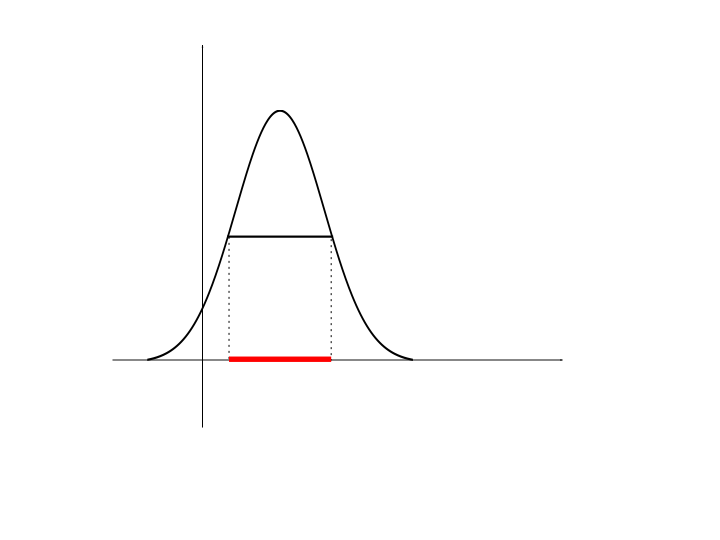
\includegraphics[scale=0.4]{\lyxdot \lyxdot /figs/normal1d}\caption{\label{fig:normal1d}}

\par\end{centering}

\end{figure}
The red line segment is centered at the mean and its width is equal
to the width of the density function at one half its peak height.

In the dynamical equations (\ref{eq:kalman-dynamics}), the state
is a point in the $x,y$ plane and therefore two dimensional. So we
need the two dimensional normal distribution. Without going into the
algebra, we may represent the two dimensional normal distribution
as shown in Figure \ref{fig:normal2d}.

\begin{figure}


\begin{centering}
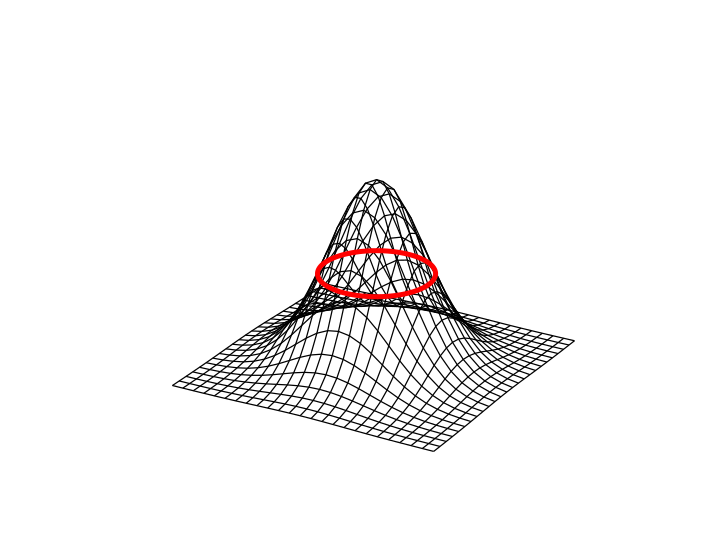
\includegraphics[scale=0.4]{\lyxdot \lyxdot /figs/normal2d}
\par\end{centering}

\begin{centering}
\caption{\label{fig:normal2d}}

\par\end{centering}

\end{figure}


In this case, the curve obtained by taking section of the probability
density function at one half its peak height is an ellipse. The center
of this ellipse is the mean of the normal distribution. 

After adopting this convention, we may think of the two dimensional
normal distribution as an ellipse in the plane. In our example, the
state $(x,y)$ is two dimensional. We do not know the state exactly
but use the normal distribution to approximate it. The particular
normal distribution we choose will be represented as an ellipse in
the $x,y$ plane.

Suppose we have an ellipse to approximate the state $(x_{n},y_{n})$.
If we move to $(x_{n+1},y_{n+1})$ following the dynamical law (\ref{eq:kalman-dynamics}),
then the ellipse is updated as in Figure \ref{fig:rotate}.

\begin{figure}
\begin{centering}
\includegraphics[scale=0.4]{\lyxdot \lyxdot /figs/rotate}
\par\end{centering}

\caption{\label{fig:rotate}}
\end{figure}


In this figure, the approximation to the state at time $n$ is the
dashed ellipse. The approximation to the state at $n+1$ is then the
solid ellipse.

The key to the Kalman filter is the way it handles the noisy observation.
The noisy observation at time $n+1$ is $z_{n+1}=y_{n+1}+\eta$, where
$\eta$ is normally distributed. The next step is to represent our
estimate of the state at time $n+1$ along with the noise in the same
picture. Following our earlier convention this representation will
be an ellipsoid as in Figure \ref{fig:add-noise}.

\begin{figure}
\begin{centering}
\includegraphics[scale=0.4]{\lyxdot \lyxdot /figs/add_noise}\caption{\label{fig:add-noise}}

\par\end{centering}

\end{figure}


The ellipse in the $x,y$, which approximated the state at time $n+1$,
has turned into an ellipsoid. The $\eta$ dimension has been added
to the $x-y$ plane.

The measured quantity is $z_{n+1}=y_{n+1}+\eta$. The known value
of $z_{n+1}$ corresponds to a plane in $x,y,\eta$ space. This plane
cuts the ellipsoid as in Figure \ref{fig:section}

\begin{figure}
\begin{centering}
\includegraphics[scale=0.4]{\lyxdot \lyxdot /figs/section}
\par\end{centering}

\caption{\label{fig:section}}


\end{figure}


The intersection of the plane with the ellipsoid is an ellipse. The
Kalman filter projects this ellipse to the $x,y$ plane, where it
becomes another ellipse. This ellipse become our updated approximation
to the state at time $n+1$, which includes the effect of the observation
$z_{n+1}$. The same process is repeated at every step. 

If you follow this picture carefully, you will notice that taking
a section of the ellipsoid and projecting to the $x,y$ plane can
shift the center of the ellipse in the $x,y$ plane. In fact the projected
ellipse may need to be enlarged to match our convention for representing
the normal distribution. 

To actually implement the Kalman filter, we must turn this picture
into algebraic formulas. That is what we now turn to.


\subsection{Current state according to Kalman}

At step $n$, the Kalman filter does not really know for sure where
the rocket is. It thinks of the current state as a pair of random
variables $X_{n},Y_{n}$ with the probability density function being
\begin{equation}
\frac{\sqrt{a_{n}c_{n}-b_{n}^{2}}}{\pi}\exp-\left(a_{n}\left(X_{n}-\mu_{n}\right)^{2}+2b_{n}\left(X_{n}-\mu_{n}\right)\left(Y_{n}-\nu_{n}\right)+c_{n}\left(Y_{n}-\nu_{n}\right)^{2}\right).\label{eq:kalman-xnyn-pdf}
\end{equation}
For this density function to make sense, the exponent must be always
negative. The discriminant of the quadratic equation implies the conditions
\begin{eqnarray*}
a_{n},c_{n} & > & 0\\
a_{n}c_{n} & > & b_{n}^{2}.
\end{eqnarray*}
We will always assume these conditions.
\begin{description}
\item [{Exercise:}] Prove that the probability density function (\ref{eq:kalman-xnyn-pdf})
is correctly normalized. To integrate it over $-\infty<X_{n},Y_{n}<\infty$,
you may start with the identity
\[
ax^{2}+2bxy+cz^{2}=a\left(x+\frac{by}{a}\right)^{2}+y^{2}\left(c-\frac{b^{2}}{a}\right).
\]

\item [{Exercise:}] Use symmetry to deduce that $\mathbb{E}X_{n}=\mu_{n}$
and $\mathbb{E}Y_{n}=\nu_{n}$.
\item [{Exercise:}] For a greater challenge with handling integrals, prove
that 
\[
\mathbb{E}\left(X_{n}-\mu_{n}\right)^{2}=\frac{a_{n}}{2\left(a_{n}c_{n}-b_{n}^{2}\right)}\quad\mathbb{\text{and}\quad E}\left(Y_{n}-\nu_{n}\right)^{2}=\frac{c_{n}}{2\left(a_{n}c_{n}-b_{n}^{2}\right)}.
\]

\end{description}
Thus the Kalman filter takes the expectation of the current position
to be $\mu_{n},\nu_{n}$. If the quantities
\[
\frac{a_{n}}{2\left(a_{n}c_{n}-b_{n}^{2}\right)},\:\frac{c_{n}}{2\left(a_{n}c_{n}-b_{n}^{2}\right)}
\]
are tiny if means we have a lot of confidence that the current state
is near $\mu_{n},\nu_{n}$. That happens for example if $a_{n},c_{n}$
are very large and $b_{n}$ is much smaller in magnitude. 


\subsection{Updating from $X_{n},Y_{n}$ to $X_{n+1},Y_{n+1}$}

The dynamical equations (\ref{eq:kalman-dynamics}) are used to update
from time $n$ to time $n+1$. Therefore the expectations of $X_{n+1},Y_{n+1}$
are as follows:
\begin{eqnarray*}
\mathbb{E}X_{n+1} & = & \mu=\frac{\mu_{n}-\nu_{n}}{\sqrt{2}}\\
\mathbb{E}Y_{n+1} & = & \nu=\frac{\mu_{n}+\nu_{n}}{\sqrt{2}}.
\end{eqnarray*}
To update the probability density function to $n+1$, we need only
make the substitution
\begin{eqnarray*}
X_{n}-\mu_{n} & = & \frac{\left(X_{n+1}-\mu\right)+\left(Y_{n+1}-\nu\right)}{\sqrt{2}}\\
Y_{n}-\nu_{n} & = & \frac{-\left(X_{n+1}-\mu\right)+\left(Y_{n+1}-\nu\right)}{\sqrt{2}}
\end{eqnarray*}
in the probability density function (\ref{eq:kalman-xnyn-pdf}). Notice
that this transformation has determinant equal to $+1$. We get the
probability density function to be 
\begin{equation}
\frac{\sqrt{ac-b^{2}}}{\pi}\exp-\left(a\left(X_{n+1}-\mu\right)^{2}+2b\left(X_{n+1}-\mu\right)\left(Y_{n+1}-\nu\right)+c\left(Y_{n+1}-\nu\right)^{2}\right).\label{eq:kalman-xn1yn1-pdf}
\end{equation}
The quantities $\mu,\nu$ were defined above. From the substitution,
we may deduce
\begin{eqnarray*}
a & = & \frac{a_{n}+c_{n}}{2}-b_{n}\\
b & = & \frac{a_{n}-c_{n}}{2}\\
c & = & \frac{a_{n}+c_{n}}{2}+b_{n}.
\end{eqnarray*}
So from thinking of the state at time $n$ using (\ref{eq:kalman-xnyn-pdf}),
the Kalman filter moves to thinking of the state at time $n+1$ using
the probability density function (\ref{eq:kalman-xn1yn1-pdf}). This
step is actually fairly trivial.


\subsection{Incorporating the observation $Z_{n+1}$}

Now comes the main idea in the Kalman filter. Once we have the probability
density function (\ref{eq:kalman-xn1yn1-pdf}), how do we update it
to reflect the measurement $Z_{n+1}$? The measurement $Z_{n+1}$,
though noisy, is our only knowledge of what is happening inside the
system. Therefore it is crucial to incorporate it correctly into our
model.

As Kalman pointed out in his 1960 paper, this is essentially a conditional
probability calculation. We know that $Z_{n+1}=Y_{n+1}+\eta$ where
$\eta$ is normally distributed with mean $0$ and variance $\sigma^{2}$.
So we may include $\eta$ with $X_{n+1},Y_{n+1}$ and write the joint
density function as:

\[
\frac{\sqrt{ac-b^{2}}}{\pi}\exp-\left(a\left(X_{n+1}-\mu\right)^{2}+2b\left(X_{n+1}-\mu\right)\left(Y_{n+1}-\nu\right)+c\left(Y_{n+1}-\nu\right)^{2}\right)\times\frac{\exp(-\eta^{2}/2\sigma^{2})}{\sqrt{2\pi}\sigma}.
\]
Here we make the substitution $\eta=Z_{n+1}-Y_{n+1}$to bring the
observation $Z_{n+1}$ into the picture. We get 
\begin{eqnarray*}
\frac{\sqrt{ac-b^{2}}}{\pi}\exp-\left(a\left(X_{n+1}-\mu\right)^{2}+2b\left(X_{n+1}-\mu\right)\left(Y_{n+1}-\nu\right)+c\left(Y_{n+1}-\nu\right)^{2}\right)\\
\times\frac{\exp(-\left(Z_{n+1}-Y_{n+1}\right)^{2}/2\sigma^{2})}{\sqrt{2\pi}\sigma}.
\end{eqnarray*}
Now comes a calculation which involves rewriting 
\[
a\left(X_{n+1}-\mu\right)^{2}+2b\left(X_{n+1}-\mu\right)\left(Y_{n+1}-\nu\right)+c\left(Y_{n+1}-\nu\right)^{2}+\frac{\left(Z_{n+1}-Y_{n+1}\right)^{2}}{2\sigma^{2}}
\]
as 
\begin{eqnarray*}
a_{n+1}\left(X_{n+1}-\mu_{n+1}\right)^{2}+2b_{n+1}\left(X_{n+1}-\mu_{n+1}\right)\left(Y_{n+1}-\nu_{n+1}\right)+c_{n+1}\left(Y_{n+1}-\nu_{n+1}\right)^{2}\\
+\text{something that depends upon \ensuremath{Z_{n+1}}but not \ensuremath{X_{n+1}}or \ensuremath{Y_{n+1}}.}
\end{eqnarray*}
For those who are comfortable with algebra, this calculation should
not be hard. Through this calculation we get that
\begin{eqnarray*}
a_{n+1} & = & a\\
b_{n+1} & = & b\\
c_{n+1} & = & c+\frac{1}{2\sigma^{2}}.
\end{eqnarray*}
In addition, $\mu_{n+1}$ and $\nu_{n+1}$ are obtained by solving
the equations 
\begin{eqnarray*}
-2a(\mu_{n+1}-\mu)-2b\left(\nu_{n+1}-\nu\right) & = & 0\\
-2b\left(\mu_{n+1}-\mu\right)-2\left(c+\frac{1}{2\sigma^{2}}\right)\left(\nu_{n+1}-\nu\right) & = & -\frac{Z_{n+1}}{\sigma^{2}}.
\end{eqnarray*}
Notice that observation $Z_{n+1}$ is making us adjust the expected
positions. 

At this point the filter equations are complete. To go from time step
$n+1$ to time step $n+2$, we repeat the same process. To begin the
filter, we may make a guess for $\mu_{0},\nu_{0}$ as well as the
parameters $a_{0},b_{0},c_{0}$. Thereafter the Kalman filter uses
the measurements $Z_{n}$ to update the estimated state at every step.

In Figure \ref{fig:Kalman} (b) and (c), the estimates for $x_{n},y_{n}$
that are graphed are the means $\mu_{n},\nu_{n}$.
\end{document}
